\section{Introduction}

In a true many-body electronic wave function, the motions of electrons are dynamically correlated across the entire range of inter-electronic distances.
A large part of this correlation is efficiently captured by various approximations to the Kohn--Sham density-functional theory (KS-DFT), which established it as a basic tool in computational chemistry and condensed-matter physics.
But the standard density functionals are semi-local in space, resulting in electron correlation energy that decays exponentially with distance---as if the electrons were essentially uncorrelated at long range (except for the special case of slowly-varying electron density).
This leads to severe underestimation of van der Waals (vdW) dispersion interactions, which are mostly caused by long-range electron correlation.
As these interactions strongly contribute to properties of nearly all biological and modern synthetic materials, many models were developed that account specifically for the long-range correlation~\cite{DionPRL04,VydrovJCP10a,JohnsonJCP06,TkatchenkoPRL09,GrimmeJCP10,AmbrosettiJCP14} to augment the semi-local (or hybrid) density-functional calculations.
This range separation of electron correlation into a short-range and long-range model can be in principle done formally~\cite{HermannCR17}, but insufficient knowledge about the ranges of different semi-local functionals prevents this in practice, leading to various semi-empirical approaches.

The SCAN functional is a recent first-principles semi-local functional~\cite{SunPRL15} with great performance across a broad range of systems in chemistry and physics, in many cases reaching the accuracy of hybrid functionals at a fraction of their cost~\cite{SunNC16}.
It is still only semi-local, however, and does not describe long-range electron correlation, and hence vdW interactions.
On the other hand, the many-body dispersion (MBD) method is a general model of long-range electron correlation~\cite{TkatchenkoPRL12,AmbrosettiJCP14} that can be combined with any short-range correlation method, such as semi-local DFT or the density-functional tight-binding method.
The crossover regime, where a short-range description blends with the long-range MBD description, is controlled with a single range-separation parameter within the MBD model.
When trying to adjust this parameter for the SCAN functional---essentially estimating the correlation range of SCAN for vdW interactions---we observed that the optimal value depends significantly on the choice of the studied systems and the choice of the optimized quantity.
Since this is not the case for other density functionals such as PBE, we set out to study in general the range of electron correlation as described by different density functionals in vdW-bound systems.

\section{Background}

\paragraph{Density functionals: Short-range correlation models}

Some aspects of the ``tail'' behaviour of semi-local density functionals in vdW systems are known, mostly from observations made on particular systems.
The Hartree--Fock (HF) model separates electron correlation into the exchange and ``pure'' correlation parts, the second of which is exclusively responsible for vdW attraction.
This does not translate well into exchange and correlation as approximated by semi-local density functionals in DFT, where the exchange part often contributes much more than the correlation part to the vdW attraction at equilibrium distances.
This behaviour is caused by the implicit cancellation of errors between the two parts, and is reflected by the fact that most of the literature on this topic is concerned with exchange, not correlation functionals.

Nearly all exchange energy functionals of the electron density, $n$, are constructed such that they are exact for the uniform electron gas, and are therefore of the form
\begin{equation}
  E_\mathrm x[n]=\int\mathrm d\mathbf rn(\mathbf r)\varepsilon^\text{unif}_\text x(n(\mathbf r))F_\mathrm x[n](\mathbf r)
  \label{eq:exchange-form}
\end{equation}
where the exchange energy density of a uniform electron gas, $\varepsilon^\text{unif}_\mathrm x(n)=-3k_\mathrm F(n)/4\pi$, $k_\mathrm F(n)(3\pi^2n)^{1/3}$, is multiplied with the so-called enhancement factor, $F_\mathrm x[n](\mathbf r)$, which goes to zero for a homogeneous density.
(This is also the reason why all such functionals describe the electron correlation energy completely in the uniform gas, including the long range part.
However, since this description is only local and effective, it does not transfer into inhomogeneous systems, which vdW-bound systems inherently are.)

The functionals studied in this work span first four rungs of the Jacob's ladder of density functionals.
The local density approximation (LDA, first rung) is defined by setting $F_\mathrm x[n]=1$~\cite{DiracMPCPS30}.
In a generalized gradient approximation (GGA, second rung), the enhancement factor depends locally on the dimensionless density gradient, $s[n]=\lvert\boldsymbol\nabla n\rvert/2k_\text F(n)n$, $F_\mathrm x[n](\mathbf r)=F^\text{GGA}_\mathrm x(s[n](\mathbf r))$, and it is the particular form of $F^\text{GGA}_\mathrm x(s)$ that distinguishes different GGAs.
Our study includes the GGA functional from Perdew, Burke, and Ernzerhof (PBE)~\cite{PerdewPRL96}.

The search for semi-local functionals with the appropriate correlation range has been done mostly within the space of GGAs and in the context of the vdW-DF non-local functional~\cite{DionPRL04,LeePRB10}, a long-range correlation method whose correlation range is not easily modified.
Several special-purpose functionals designed to combine well with long-range correlation models were developed, ranging from completely new constructions~\cite{PernalPRL09,WellendorffPRB12}, to recombinations of older forms~\cite{CooperPRB10,HamadaPRB14,BerlandPRB14}, to simple reparameterizations of standard functionals~\cite{ZhangPRL98,KlimesJPCM10,KlimesPRB11}.
(An ``ideal'' exchange functional in this regard would be different from the exact exchange, because it would still contain a part of the short-range post-HF correlation that is not covered by GGA correlation functionals.)
All of these functionals perform well for vdW-bound systems (when combined with a vdW model), but not much is known about their accuracy for other systems, preventing them from becoming general methods.

In meta-GGAs, the third rung of the Jacob's ladder, still higher derivatives of the electron density (or occupied orbitals, $\phi_i$) beyond the gradient are used to construct the enhancement factor, $F_\mathrm x$.
This includes the Laplacian of the density and the KS kinetic energy density, $\tau[n]=\sum_i^\text{occ}\lvert\boldsymbol\nabla\phi_i\rvert^2/2$.
Two meta-GGAs are included in this study: TPSS~\cite{TaoPRL03} and the already mentioned SCAN\@.
In both of them (and in SCAN only so), the kinetic energy density enters via a local density parameter, $\alpha[n](\mathbf r)$, that serves as a measure of localization of electrons~\cite{BeckeJCP90},
\begin{equation}
\alpha=(\tau-\tau^\text W)/\tau^\text{unif}\geq0
\end{equation}
where $\tau^\text W[n]=\lvert\boldsymbol\nabla n\rvert^2/8n$ is the von Weizsäcker kinetic energy functional, exact for single-orbital electron densities, and $\tau^\text{unif}(n)=3k_\text F(n)^2n/10$ is the Thomas--Fermi kinetic energy functional, exact for the uniform electron gas.
This parameter can distinguish different kinds of electron density~\cite{SunPRL13}: $\alpha\approx0$ where a single orbital dominates the electron density, $\alpha\approx1$ for a slowly varying (metallic) electron density, and $\alpha\gg1$ where two closed-shell electron densities overlap, which is characteristic of vdW-bound systems in equilibrium (and to lesser degree also for inter-shell regions within atoms and molecules~\cite{BeckeJCP90}).

The fourth rung of functionals contains GGAs and meta-GGAs with partial admixture of exact exchange, which is a nonlocal functional of the occupied orbitals.
As in HF, exact exchange does not contribute to the vdW attraction at any distance, but substantially improves accuracy of (meta-)GGAs for many chemical problems. % chktex 36
Here, we study the hybrid GGAs PBE0~\cite{AdamoJCP99} and B3LYP~\cite{BeckeJCP93}, and a hybrid meta-GGA M06~\cite{ZhaoTCA08}.
We also briefly look at SCAN0~\cite{HuiJCP16}, a PBE0-like version of SCAN with 25\% of exact exchange.

We do not include the fifth-rung functionals, such as the random-phase approximation or double-hybrid functionals, because they already contain long-range electron correlation by construction, at the price of much increased computational cost.

\paragraph{Van der Waals methods: Long-range correlation models}

By construction, density functionals from the first four rungs cannot describe long-range electron correlation.
We use here three different vdW methods that correct for this deficiency by complementing short-range correlation described by the functionals.
All three have some explicit form of range separation built into them, which enables us to use them as probes to examine the implicit correlation range of the functionals.
Hence, we briefly review the range-separation mechanisms in these vdW methods.

MBD is a many-body coarse-grained model of long-range electron correlation based on density-dependent atomic polarizabilities and a dipole potential in place of the electronic Coulomb potential.
To avoid double counting of the electron correlation at short range where the density functionals describes it (and are much better at that job any long-range model would be), the dipole potential is damped, and the onset of this damping is controlled via a single parameter, $\beta^\text{MBD}$, that relates to atomic vdW radii.

The nonlocal functional of Vydrov and Van Voorhis (VV10)~\cite{VydrovJCP10a} is a point-pairwise long-range correlation model based on a local effective polarizability functional of the electron density.
Here, the mechanism for damping works by reducing the polarizability at two interacting points if they are too close, and the parameter controlling the range, $b^\text{VV10}$, relates to the magnitude of the local effective polarizability.

The D3 method by Grimme~\cite{GrimmeJCP10} is a pairwise (or three-body) coarse-grained vdW model based on atomic polarizabilities derived from local atomic structure and damped dipole--dipole and dipole--quadrupole potentials.
The particular form of damping in D3 received some attention~\cite{GrimmeJCC11,SchroderJCTC15,SmithJPCL16,WitteJCTC17}, and of the two main variants (both based on atomic vdW radii), the original one is similar to that used in MBD, whereas the other, originally from Johnson and Becke (BJ)~\cite{JohnsonJCP06}, has a different limiting behaviour at short range.
Since our goal here is to cover a broad range of vdW models, we use the BJ damping for its distinction from the damping used in MBD\@.
The BJ-damped D3 method uses three parameters that control its short-range behaviour: $s_8^\text{D3}$ controls global mixing of the dipole--quadrupole term (which is inherently short-range), and the closely related $a_1^\text{D3}$ and $a_2^\text{D3}$ control the onset of the dipole--dipole term ($a_1^\text{D3}$ scales vdW radii, $a_2^\text{D3}$ offsets them).

\paragraph{Van der Waals benchmark sets}

Whereas the vdW models have explicit correlation range, the range of density functionals is only implicit, and the combined DFT+vdW models are therefore constructed by optimizing the range separation in vdW models against some benchmark properties, usually binding or lattice energies.
Several benchmark sets of vdW-bound systems have been established, of which we use predominantly three: the S66 set of 66 smaller organic dimers~\cite{RezacJCTC11}, the X23 set of 23 molecular crystals~\cite{ReillyJCP13}, and the S12L set of 12 large supramolecular complexes~\cite{RisthausJCTC13}.
The S66 set is especially useful here, because each of the 66 dimers is calculated at 8 intermolecular distances distributed around the equilibrium distance.

The raw results of evaluating a method on a benchmark set consist of the distribution of errors, $E_i-E_i^\text{ref}$.
Since the interaction energies in vdW systems span orders of magnitude, we use relative errors, $\Delta_\mathrm rE_i=(E_i-E_i^\text{ref})/(-E_i^\text{ref})$ (assuming $E_i$ are negative).
The comparison of error distributions between different methods is simplified by introducing various statistical measures.
A popular measure is the mean absolute relative error (MARE), $\sum_i\lvert\Delta_\mathrm rE_i\rvert/N$, which serves well as a single-number indicator of performance, but does not provide much insight into the actual error distribution.
Instead, we use the mean relative error (MRE), $\sum_i\Delta_\mathrm rE_i/N$, and the standard deviation of the relative errors (SDRE),
\[ \text{SDRE}=\frac1N\sqrt{\sum_i(\Delta_\mathrm rE_i-\text{MRE})^2} \]
This enables us to study both the systematic error of a method represented by MRE (overall underbinding or overbinding), as well as the ``statistical'' error represented by SDRE (how consistent a method is).

\section{Results}

Figure 1.\ shows the distributions of relative errors in binding energies on the S66x8 set of six different functionals (LDA, PBE, PBE0, B3LYP, SCAN, M06) combined with the MBD method.
The values of the damping parameter $\beta$

Figure 2.\ shows the dependency of the systematic and statistical errors on the respective damping parameters of three

Figure 1 shows the distributions of relative errors in binding energies across the intermolecular distances for several functionals combined with MBD at different values of the range-separation parameter $\beta$.
The LDA functional without any long-range tail (LDA, no vdW) overbinds at short range and underbinds at long range, caused by the notorious vdW binding of LDA for the ``wrong'' reasons.
The binding caused by the LDA exchange decays quickly, so the long-range behaviour can be corrected well in LDA+MBD (LDA, $\beta=1.4$), however, the short-range behaviour is irreparable.
In contrast, PBE+MBD (PBE, $\beta=0.83$) has a consistent behaviour across all distances, with the mean error being close to zero, and only the error variance increasing monotonously for shorter distances.
PBE0+MBD (PBE, $\beta=0.83$) behaves very similarly to PBE+MBD, only with the error variance being somewhat reduced (but not the outliers).
B3LYP, another hybrid GGA, is much more repulsive, and the optimal range separation is shorter (B3LYP, $\beta=0.67$).
This does not necessarily mean that B3LYP is short-range though, and indeed B3LYP is still significantly repulsive even at the $\times$2 distances (cf.\ LDA).
Furthermore, the error variance is significantly increased compared to PBE+MBD\@.
This is caused for a large part by B3LYP underbinding hydrogen-bonded complexes even more than other binding patterns.
Making the range separation in B3LYP+MBD even shorter than $\beta=0.67$ does not lead to further improvement.
For the SCAN functional, we plot the error distributions for two distinct range separations, $\beta=1.1$ and $\beta=1.4$, minimizing the error variance and absolute mean error, respectively.
As we show below, these two optimizations roughly coincide for PBE, but they do not for SCAN\@.

The distributions of binding energy errors across a benchmark set and their dependence on 

\begin{figure*}
\makebox[\textwidth][c]{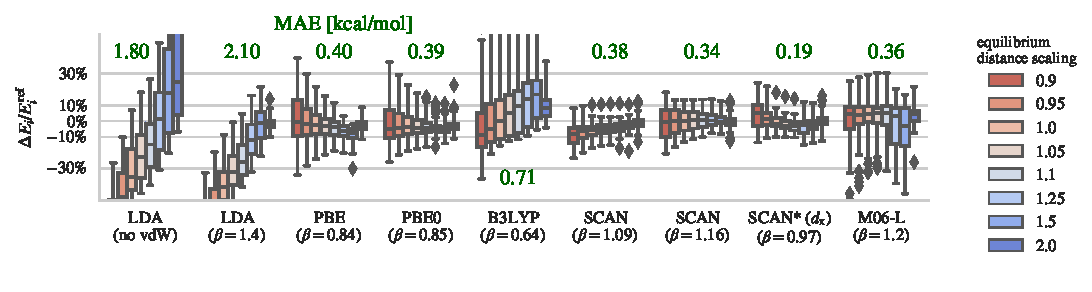
\includegraphics{../media/s66-dists}}
\caption{\textbf{Label.} Text.
}\label{fig:s66-dists}
\end{figure*}

\begin{figure*}
\makebox[\textwidth][c]{
\begin{tikzpicture}
\node [below right] at (0,0) {\bfseries a};
\node [below right] at (0,0) {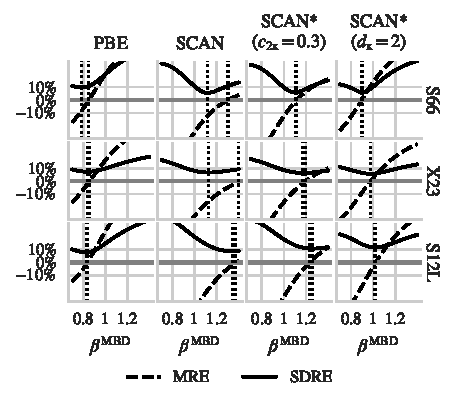
\includegraphics{../media/mbd-param-fitting.pdf}};
\node [below right] at (9.5,0) {\bfseries b};
\node [below right] at (9.5,0) {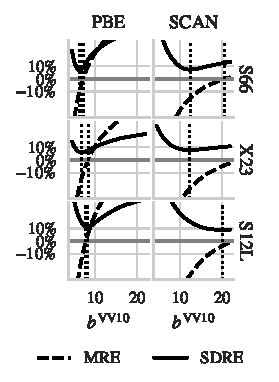
\includegraphics{../media/vv10-param-fitting.pdf}};
\node [below right] at (14.7,0) {\bfseries c};
\node [below right] at (14.7,0) {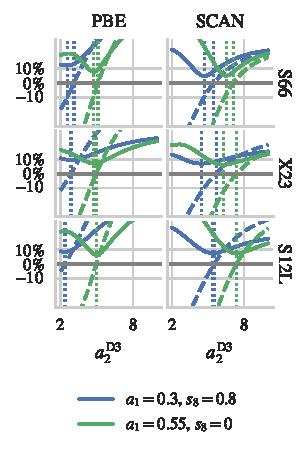
\includegraphics{../media/d3-param-fitting.pdf}};
\end{tikzpicture}
}
\caption{\textbf{Label.} Text.
}\label{fig:param-fitting}
\end{figure*}

\begin{figure}
\centering
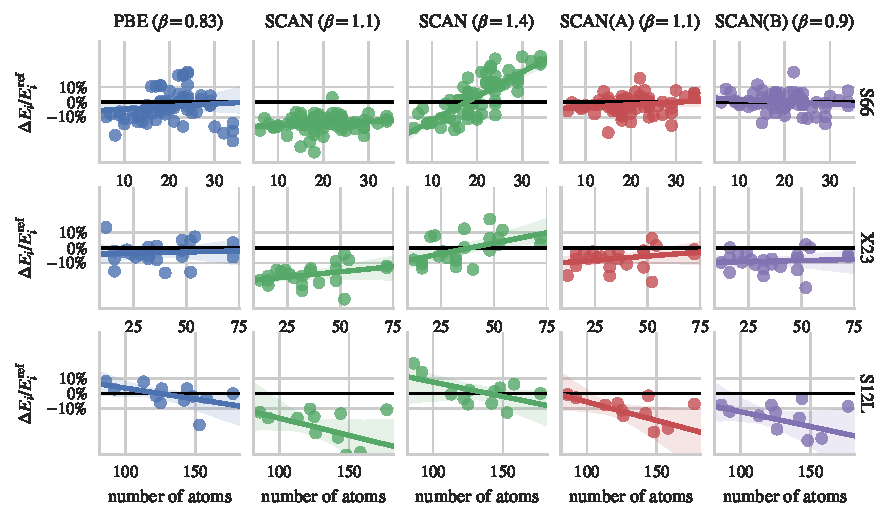
\includegraphics{../media/size-dependence}
\caption{\textbf{Label.} Text.
}\label{fig:size-dependence}
\end{figure}

\begin{figure}

\centering
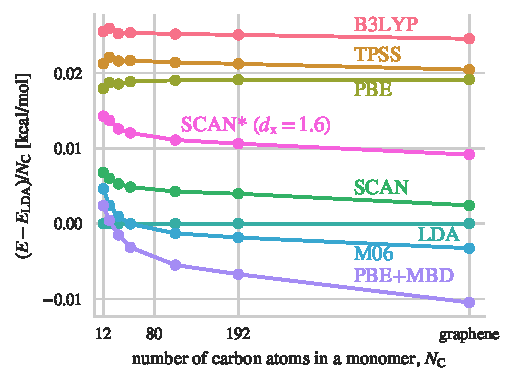
\includegraphics{../media/flakes}
\caption{\textbf{Label.} Text.
}\label{fig:flakes}
\end{figure}

\section{Conclusions}

\paragraph{Calculation details}
